
%%%%% DONT CHANGE ANYTHING BEFORE THE "TITLE" SECTION.%%%%%
\documentclass{article} % Especially this!
% _____        _____ _  __          _____ ______  _____ 
%|  __ \ /\   / ____| |/ /    /\   / ____|  ____|/ ____|
%| |__) /  \ | |    | ' /    /  \ | |  __| |__  | (___  
%|  ___/ /\ \| |    |  <    / /\ \| | |_ |  __|  \___ \ 
%| |  / ____ \ |____| . \  / ____ \ |__| | |____ ____) |
%|_| /_/    \_\_____|_|\_\/_/    \_\_____|______|_____/ 
%%%%%%%%%%%%%%%%%%%%%%%%%%%%%%%%%%%%%%%%%%%%%%%%%%%%%%%%

\usepackage[english]{babel}
\usepackage[utf8]{inputenc}
\usepackage[margin=1.5in]{geometry}
\usepackage{amsmath}
\usepackage{amsthm}
\usepackage{amsfonts}
\usepackage{amssymb}
\usepackage[usenames,dvipsnames]{xcolor}
\usepackage{graphicx}
\usepackage[siunitx]{circuitikz}
\usepackage{tikz}
\usepackage[colorinlistoftodos, color=orange!50]{todonotes}
\usepackage{hyperref}
\usepackage[numbers, square]{natbib}
\usepackage{fancybox}
\usepackage{epsfig}
\usepackage{soul}
\usepackage[framemethod=tikz]{mdframed}
\usepackage[shortlabels]{enumitem}
\usepackage[version=4]{mhchem}
\usepackage{multicol}



%%%%%%%%%%%%%%%%%%%%%%%%%%%%%%%%%%%%%%%%%%%%%%%%%%%%%%%


%   _____ _    _  _____ _______ ____  __  __ 
%  / ____| |  | |/ ____|__   __/ __ \|  \/  |
% | |    | |  | | (___    | | | |  | | \  / |
% | |    | |  | |\___ \   | | | |  | | |\/| |
% | |____| |__| |____) |  | | | |__| | |  | |
%  \_____|\____/|_____/   |_|  \____/|_|  |_|
%%%%%%%%%%%%%%%%%%%%%%%%%%%%%%%%%%%%%%%%%%%%%%%%
%  _____ ____  __  __ __  __          _   _ _____   _____ 
% / ____/ __ \|  \/  |  \/  |   /\   | \ | |  __ \ / ____|
%| |   | |  | | \  / | \  / |  /  \  |  \| | |  | | (___  
%| |   | |  | | |\/| | |\/| | / /\ \ | . ` | |  | |\___ \ 
%| |___| |__| | |  | | |  | |/ ____ \| |\  | |__| |____) |
% \_____\____/|_|  |_|_|  |_/_/    \_\_| \_|_____/|_____/ 
%%%%%%%%%%%%%%%%%%%%%%%%%%%%%%%%%%%%%%%%%%%%%%%%%%%%%%%%%%




% SYNTAX FOR NEW COMMANDS:
%\newcommand{\new}{Old command or text}

%%%JAVA CODE
\usepackage{listingsutf8}
\definecolor{dkgreen}{rgb}{0,0.6,0}
\definecolor{javadocblue}{rgb}{0.25,0.35,0.75} % javadoc
\definecolor{gray}{rgb}{0.5,0.5,0.5}
\definecolor{mauve}{rgb}{0.58,0,0.82}

\lstdefinestyle {javacode}
{ %
  language=Java,                  % the language of the code
 % inputencoding=latin1,			  % input encod. 
  inputencoding=utf8/latin1,			  % input encod. 
  basicstyle=\footnotesize,       % the size of the fonts that are used for the code
  numbers=left,                   % where to put the line-numbers
  numberstyle=\tiny\color{gray},  % the style that is used for the line-numbers
  stepnumber=1,                   % the step between two line-numbers. If it's 1, each line 
                                  % will be numbered
  numbersep=5pt,                  % how far the line-numbers are from the code
  backgroundcolor=\color{white},  % choose the background color. You must add \usepackage{color}
  showspaces=false,               % show spaces adding particular underscores
  showstringspaces=false,         % underline spaces within strings
  showtabs=false,                 % show tabs within strings adding particular underscores
  frame=single,                   % adds a frame around the code
  rulecolor=\color{black},        % if not set, the frame-color may be changed on line-breaks within not-black text (e.g. commens (green here))
  tabsize=4,                      % sets default tabsize to 2 spaces
  captionpos=b,                   % sets the caption-position to bottom
  breaklines=true,                % sets automatic line breaking
  breakatwhitespace=false,        % sets if automatic breaks should only happen at whitespace
  title=\lstname,                 % show the filename of files included with \lstinputlisting;
                                  % also try caption instead of title
  keywordstyle=\color{blue},          % keyword style
  commentstyle=\color{dkgreen},       % comment style
  morecomment=[s][\color{javadocblue}]{/**}{*/},
  stringstyle=\color{mauve},         % string literal style
  escapeinside={\%*}{*)},            % if you want to add a comment within your code
  morekeywords={*,...}               % if you want to add more keywords to the set
}


% the following is needed for syntax highlighting
\usepackage{color}
% this is needed for forms and links within the text
\usepackage{hyperref}

%%%PSEUDO_CODICE
\usepackage{algorithm}
\usepackage[noend]{algpseudocode}

%%%SUB-PACKAGES
\usepackage{subcaption}

%%%HEADER SEZIONI
\usepackage{fancyhdr}
\setlength{\headheight}{15pt}
\pagestyle{fancy}
\renewcommand{\sectionmark}[1]{\markright{\thesection\ - #1}}
\fancyhf{}
\rhead{\fancyplain{}{\thepage}}
\lhead{\fancyplain{}{\rightmark }} 

%%%NOTAZIONE COMPLESSITÀ
\usepackage{fourier}
\DeclareMathAlphabet{\mathcal}{OMS}{cmsy}{m}{n}
\SetMathAlphabet{\mathcal}{bold}{OMS}{cmsy}{b}{n}

%%%Usato per posizionare le immagini
\usepackage{float}

%%%Footnote nella stessa pagina
\interfootnotelinepenalty=10000





\newcommand{\blah}{blah blah blah \dots}

%%%%%%%%%%%%%%%%%%%%%%%%%%%%%%%%%%%%%%%%%%%%%%%%%%%%%%%%%
%  _______ ______          _____ _    _ ______ _____  	%
% |__   __|  ____|   /\   / ____| |  | |  ____|  __ \ 	%
%    | |  | |__     /  \ | |    | |__| | |__  | |__) |	%
%    | |  |  __|   / /\ \| |    |  __  |  __| |  _  / 	%
%    | |  | |____ / ____ \ |____| |  | | |____| | \ \ 	%
%    |_|  |______/_/    \_\_____|_|  |_|______|_|  \_\	%
%%%%%%%%%%%%%%%%%%%%%%%%%%%%%%%%%%%%%%%%%%%%%%%%%%%%%%%%%
%														%
% 			COMMANDS				SUMMARY				%
% \clarity{points}{comment} >>> "Clarity of Writing"	%
% \other{points}{comment}	>>> "Other"					%
% \spelling{comment}		>>> "Spelling"				%
% \units{comment}			>>> "Units"					%
% \english{comment}			>>> "Syntax and Grammer"	%
% \source{comment}			>>> "Sources"				%
% \concept{comment}			>>> "Concept"				%
% \missing{comment}			>>> "Missing Content"		%
% \maths{comment}			>>> "Math"					%
% \terms{comment}			>>> "Science Terms"			%
%														%
%%%%%%%%%%%%%%%%%%%%%%%%%%%%%%%%%%%%%%%%%%%%%%%%%%%%%%%%%
\setlength{\marginparwidth}{3.4cm}


% NEW COUNTERS
\newcounter{points}
\setcounter{points}{100}
\newcounter{spelling}
\newcounter{english}
\newcounter{units}
\newcounter{other}
\newcounter{source}
\newcounter{concept}
\newcounter{missing}
\newcounter{math}
\newcounter{terms}
\newcounter{clarity}
\newcounter{late}

% COMMANDS

\newcommand{\late}{\todo{late submittal (-5)}
	\addtocounter{late}{-5}
	\addtocounter{points}{-5}}

\definecolor{pink}{RGB}{255,182,193}
\newcommand{\hlp}[2][pink]{ {\sethlcolor{#1} \hl{#2}} }

\definecolor{myblue}{rgb}{0.668, 0.805, 0.929}
\newcommand{\hlb}[2][myblue]{ {\sethlcolor{#1} \hl{#2}} }

\newcommand{\clarity}[2]{\todo[color=CornflowerBlue!50]{CLARITY of WRITING(#1) #2}\addtocounter{points}{#1}
	\addtocounter{clarity}{#1}}

\newcommand{\other}[2]{\todo{OTHER(#1) #2} \addtocounter{points}{#1} \addtocounter{other}{#1}}

\newcommand{\spelling}{\todo[color=CornflowerBlue!50]{SPELLING (-1)} \addtocounter{points}{-1}
	\addtocounter{spelling}{-1}}
\newcommand{\units}{\todo{UNITS (-1)} \addtocounter{points}{-1}
	\addtocounter{units}{-1}}

\newcommand{\english}{\todo[color=CornflowerBlue!50]{SYNTAX and GRAMMAR (-1)} \addtocounter{points}{-1}
	\addtocounter{english}{-1}}

\newcommand{\source}{\todo{SOURCE(S) (-2)} \addtocounter{points}{-2}
	\addtocounter{source}{-2}}
\newcommand{\concept}{\todo{CONCEPT (-2)} \addtocounter{points}{-2}
	\addtocounter{concept}{-2}}

\newcommand{\missing}[2]{\todo{MISSING CONTENT (#1) #2} \addtocounter{points}{#1}
	\addtocounter{missing}{#1}}

\newcommand{\maths}{\todo{MATH (-1)} \addtocounter{points}{-1}
	\addtocounter{math}{-1}}
\newcommand{\terms}{\todo[color=CornflowerBlue!50]{SCIENCE TERMS (-1)} \addtocounter{points}{-1}
	\addtocounter{terms}{-1}}


\newcommand{\summary}[1]{
	\begin{mdframed}[nobreak=true]
		\begin{minipage}{\textwidth}
			\vspace{0.5cm}
			\begin{center}
				\Large{Grade Summary} \hrule 
			\end{center} \vspace{0.5cm}
			General Comments: #1
			
			\vspace{0.5cm}
			Possible Points \dotfill 100 \\
			Points Lost (Late Submittal) \dotfill \thelate \\
			Points Lost (Science Terms) \dotfill \theterms \\
			Points Lost (Syntax and Grammar) \dotfill \theenglish \\
			Points Lost (Spelling) \dotfill \thespelling \\
			Points Lost (Units) \dotfill \theunits \\
			Points Lost (Math) \dotfill \themath \\
			Points Lost (Sources) \dotfill \thesource \\
			Points Lost (Concept) \dotfill \theconcept \\
			Points Lost (Missing Content) \dotfill \themissing \\
			Points Lost (Clarity of Writing) \dotfill \theclarity \\
			Other \dotfill \theother \\[0.5cm]
			\begin{center}
				\large{\textbf{Grade:} \fbox{\thepoints}}
			\end{center}
		\end{minipage}
\end{mdframed}}

%#########################################################

%To use symbols for footnotes
%\renewcommand*{\thefootnote}{\fnsymbol{footnote}}
%To change footnotes back to numbers uncomment the following line
%\renewcommand*{\thefootnote}{\arabic{footnote}}

% Enable this command to adjust line spacing for inline math equations.
% \everymath{\displaystyle}

% _______ _____ _______ _      ______ 
%|__   __|_   _|__   __| |    |  ____|
%   | |    | |    | |  | |    | |__   
%   | |    | |    | |  | |    |  __|  
%   | |   _| |_   | |  | |____| |____ 
%   |_|  |_____|  |_|  |______|______|
%%%%%%%%%%%%%%%%%%%%%%%%%%%%%%%%%%%%%%%


\title{
	\normalfont \normalsize 
		\textsc{\textbf{UNIVERSITÀ DEGLI STUDI DI TORINO} \\ 
		Master's Degree in Computer Science} \\
	[10pt] 
	\rule{\linewidth}{0.5pt} \\[6pt] 
	\large Esercizio 1: Traduttore transfer sintattico IT-EN\\
	\rule{\linewidth}{2pt}  \\[10pt]
}
\author{Diego Ercoli}
\date{\today}

\begin{document}
	
	\maketitle
	\noindent
	Docente \dotfill Prof. Alessandro Mazzei \\
	Corso \dotfill Tecnologie del linguaggio naturale  \\

	
	%\begin{abstract} Prova	\end{abstract}	
		
%	\tableofcontents
	%%%%%%%%%%%%%%%%%%%%%%%%%%%%%%

	\section{Obiettivi}
Questa esercitazione mira ad implementare un traduttore automatico
dall'italiano all'inglese basato su \textit{Trasfer Sintattico}\footnote{Approccio simbolico ben noto in letteratura definito da Vaquois nel suo triangolo\cite{book}}.
\begin{figure}[ht]
	\centering 
	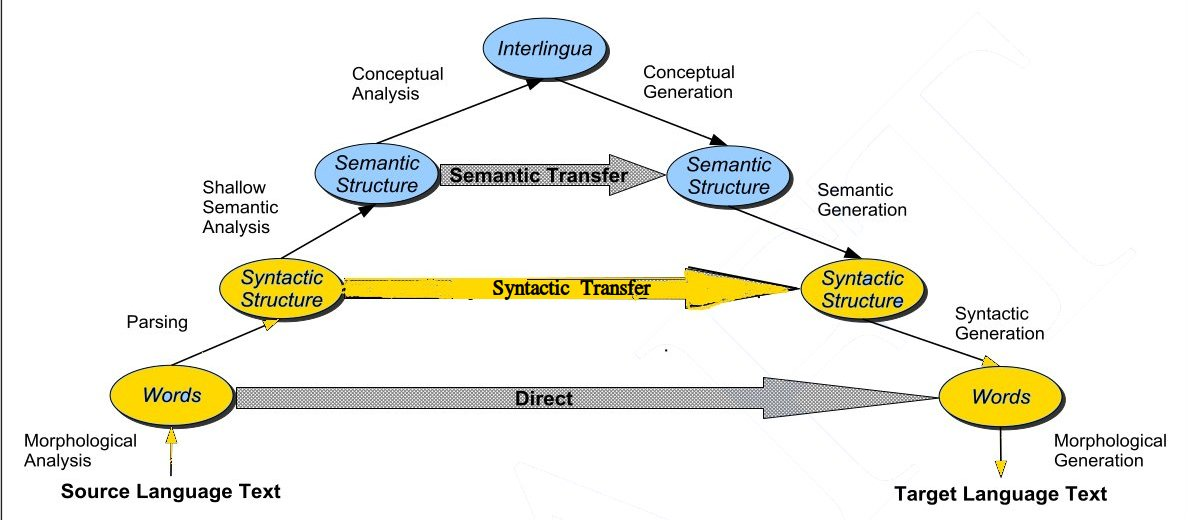
\includegraphics[scale=0.25]{./img/TransferSintattico}
	\caption{Il triangolo di Vauquois (1968)}
	\label{Vauquois_triangle}
\end{figure}\\
Come evidenziato in Figura \ref{Vauquois_triangle}, il processo sotteso al suddetto paradigma consta 
nell'analizzare morfologicamente la frase in input, costruire il relativo albero di parsing, applicare ad esso opportune regole di trasformazione volte alla costruzione di una struttura sintattica per la lingua target, ponendo quindi le basi per la generazione della frase tradotta. \\
Ciascuna fase del processo verrà analizzata nel dettaglio nelle successive sezioni, prestando particolare attenzione alle strutture dati impiegate ed ai dettagli implementativi rilevanti. L'intera pipeline di elaborazione è stata implementata
nel linguaggio Java. 

\subsection{Requisiti}
\label{sec:requisiti}
La Traduzione automatica è un task intrinsecamente difficile, ancora oggi i moderni traduttori non sono in grado si svolgere pienamente quella \textit{letteraria} \cite{book}. \\
L'esercitazione  si pone l'obiettivo di costruire un applicativo in grado di elaborare un numero ben ristretto di frasi della lingua italiana, a tal proposito vengono riportate le specifiche dei vincoli che devono essere soddisfatti dall'input:
\begin{itemize}[label=$\ast$]
	\item Il periodo in ingresso deve essere mono-proposizionale\footnote{Il periodo deve essere composto da una sola proposizione, non sono pertanto ammesse proposizioni subordinate} 
	\item La frase deve essere affermativa
	\item Il verbo deve essere coniugato al modo Indicativo
	\item L'avverbio deve essere un modificatore del verbo
	\item La frase non deve contenere congiunzioni
%	\item L'aggettivo non può essere un modificatore dell'avverbio
	\item I \textbf{lemmi} dei termini della frase devono appartenere al seguente lessico:
	\lstinputlisting[label={lexicon},style = javacode, caption ={Lessico accettato per l'Italiano}]{java/lexicon}  
	
	
\end{itemize}
La violazione di uno o più dei suddetti vincoli comporterà il lancio di un'eccezione custom da parte dell'applicativo. \\
Il programma deve essere dunque in grado di elaborare le seguenti frasi:
\begin{enumerate}[label=(\roman*)]
	\item È la spada-laser di tuo padre
	\item Ho fatto una mossa leale
	\item Gli ultimi avanzi della vecchia Repubblica sono stati spazzati via
\end{enumerate}



	\section{Analisi}
La prima fase del processo di traduzione consta nell'eseguire l'analisi morfologica e sintattica della frase inserita dall'utente (Figura \ref{Vauquois_triangle}). \\
A tal fine, si è fatto uso delle API offerte dal progetto open-source Tint \cite{tint_due}.
Si sono sperimentate due modalità di interazione:
\begin{enumerate}
	\item Importazione libreria Java ed uso delle relative API\footnote{Per maggiori dettagli si rimanda il lettore alla sezione \textit{TINT Java API }della pagina: https://dh.fbk.eu/research/tint/download-and-usage/}
		\item Chiamata API REST al WebService di Tint, specificando nel body della richiesta HTTP la frase da processare.
		In Figura \ref{REST} viene mostrato come costruire la richiesta utilizzando l'applicativo Postman \footnote{Applicativo client utilizzabile per testare API REST (https://www.postman.com/)} ed il command line tool CURL\footnote{Strumento con interfaccia a riga di comando utilizzabile per trasferire dati attraverso la rete}. \\
		In questo modo si può dunque sviluppare applicativi di NLP senza essere legati all'utilizzo del linguaggio di programmazione Java, tuttavia i tempi di elaborazione possono essere influenzati dalla connessione di rete.
\end{enumerate}
	\begin{figure}[!ht]
	\centering
	\subcaptionbox{Client Postman}{%
		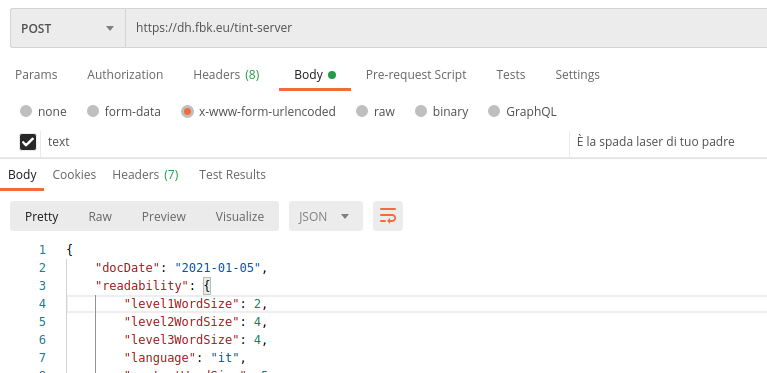
\includegraphics[width=0.75\textwidth]{./img/REST_Postman}%
	}\par\medskip
	\subcaptionbox{CURL}{%
		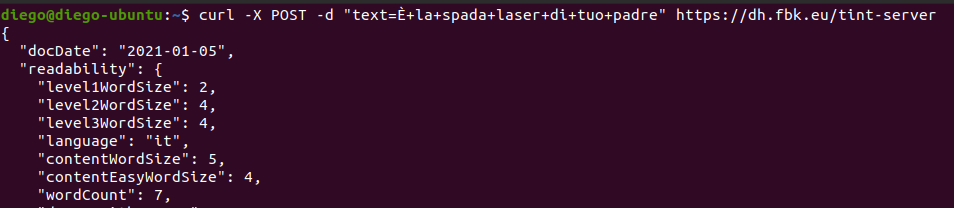
\includegraphics[width=0.75\textwidth]{./img/REST_CURL}%
	}
	\caption{Chiamata REST al server di Tint e successiva HTTP Response contenente dati in formato JSON}
	\label{REST}
\end{figure}
Indipendentemente dal tipo di interazione scelta, in entrambi i casi Tint restituisce in formato JSON il risultato della sua pipeline di elaborazione che comprende: segmentazione del testo in tokens, analisi morfologica ed individuazione dei morfemi, POS tagging, lemmatizzazione,  dependency parsing. \\
Analizzando il contenuto del JSON in questione, tra i vari dati è possibile notare la presenza di due JSONArray:
\begin{itemize}
	\item array "\textit{tokens}": 
	è il risultato della segmentazione del testo in \textbf{N tokens}\footnote{Nel seguito con le espressioni "parole della frase" o "elementi lessicali della frase" faremo riferimento ai suddetti tokens}.
	Ciascun elemento ha come attributi il lemma, il POS, l'insieme di morfermi, ... etc. Sono inoltre esplicitate in un sotto-array delle features linguistiche in relazione al valore del POS: genere e numero nel caso di un nome, tempo verbale nel caso di un verbo, ... etc.
	\item array "\textit{basic-dependencies}": è il risultato dell'analisi sintattica, più nello specifico del parsing a dipendenze. L'array contiene le \textbf{N-1 dipendenze}\footnote{Relazioni grammaticali binarie dirette tra gli elementi lessicali della frase.}, per ciascuna vengono specificati: 
		\begin{itemize}[label=$\ast$]
			\item indice $i\in[1,N]$ che punta alla parola della frase che funge da \textbf{testa}
			\item indice $j\in[1,N] \; (j \neq i) $ che punta alla parola che funge da \textbf{dipendente}
			\item etichetta della relazione
		\end{itemize}
	Nell'array è presente inoltre una relazione fittizia con etichetta "ROOT" che identifica la parola che costituisce la testa della frase (radice dell'albero).
\end{itemize}


Come verrà discusso nella Sezione {\ref{sec:transfer}}, nella fase di \textit{Transfer Sintattico} sarà necessario attraversare l'albero a dipendenze dalla radice verso le foglie, passando per i vari nodi intermedi.
Dato un nodo, dobbiamo disporre di opportuni puntatori che ci consentano di ottenere la lista dei nodi figli in tempo $\mathcal{O}(1)$ e di poter effettuare quindi la visita in ampiezza in tempo $\mathcal{O}(N)$;  cosa che risulterebbe impraticabile se utilizzassimo come struttura dati direttamente l'array \textit{basic-dependencies} di Tint (per ogni nodo visitato, l'insieme dei suoi figli sarebbero prelevati ogni volta in tempo $\mathcal{O}(N)$, un'ipotetica visita dell'albero in ampiezza richiederebbe quindi un tempo $\mathcal{O}(N^2)$). \\
Di conseguenza, a partire dall'array di relazioni di dipendenze sopra citato, viene costruita una struttura dati ad Albero con un numero arbitrario di figli (Figura \ref{tree}).
\begin{figure}[ht]
	\centering 
	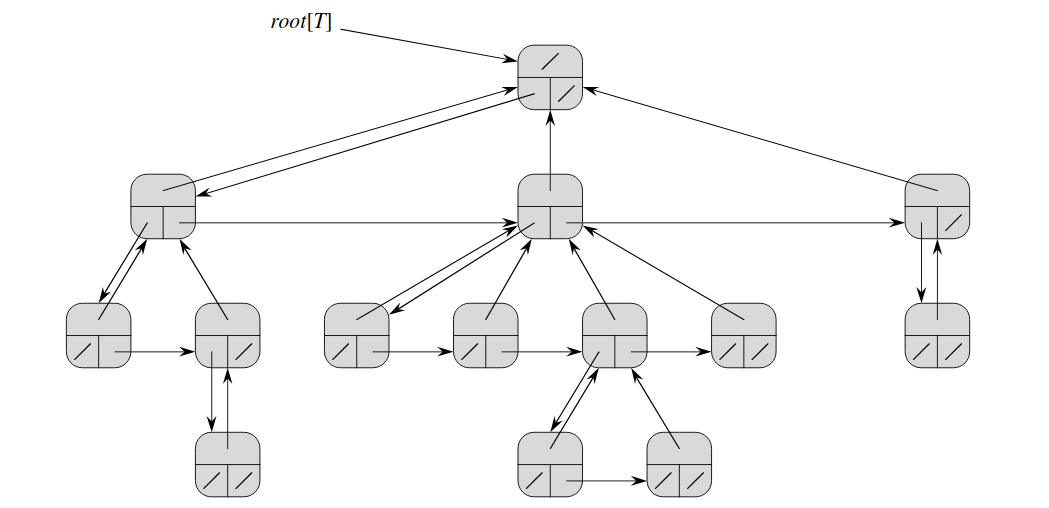
\includegraphics[scale=0.35]{./img/Albero}
	\caption{Rappresentazione intuitiva struttura dati ad albero.}
	\label{tree}
\end{figure}
\lstinputlisting[label={tree_code},style = javacode, caption ={Implentazione in Java struttura dati albero con numero arbitrario di figli. }]{java/Tree.java}
Nel Listing \ref{parsing_code} vengono riportati i dettagli relativi al processo di parsing e di generazione della struttura dati ad albero.
Ogni nodo dell'albero, corrispondente in maniera biunivoca ad una parola $i$ della frase, viene dotato di un puntatore "aggiuntivo" ad un oggetto di tipo \textit{MorphSyntaxInfo} che incapsula le informazioni morfologiche della parola in questione, provenienti dagli attributi dell'elemento $i$ dell'array "tokens" di Tint precedentemente descritto. 
Per ogni relazione di dipendenza, il nodo corrispondente al dipendente viene aggiunto alla lista dei figli del nodo corrispondente alla testa della relazione. \\
Al termine del processo restituiamo l'albero appena creato, che incorpora tutte le informazioni morfo-sintattiche della frase che potranno essere acquisite e processate visitando l'albero 
a partire dalla radice (testa della frase).



\lstinputlisting[label={parsing_code},style = javacode, caption ={Creazione \textbf{albero a dipendenze} a partire dalla frase in ingresso. }]{java/Parser.java}







%\item Vengono riconosciute solo le seguenti relazioni di dipendenza:
% \lstinputlisting[style = javacode, caption ={}]{java/deprel}
%\item I POS\footnote{acronimo di Part of Speech} riconosciuti ed analizzati sono esplicitati nella seguente enumerazione:
%\lstinputlisting[style = javacode, caption ={}]{java/pos}  
	\section{Transfer}
\label{sec:transfer}
Una volta ottenuto l'albero di parsing per la frase nella lingua sorgente,
dobbiamo disporre di opportune regole/fonti di conoscenza che ci consentano di attuare 
il Transfer lessicale e sintattico.
\subsection{Transfer lessicale}
Denotiamo con $I$ il lessico \ref{lexicon} dichiarato nella Sottosezione \ref{sec:requisiti}.Possiamo notare come non tutti i lemmi siano monosemici. Il caso più evidente è dato dal verbo polisemico "fare", il quale in relazione al contesto può assumere un significato (\textit{senso}) differente. In Figura vengono riportate due possibili accezioni ottenute consultando la risorsa Babelnet, che evidenziano come la traduzione debba avvenire sulla base del particolare senso del lemma. 
	\begin{figure}[ht]
		\centering
		\begin{subfigure}{.5\textwidth}
			\centering
			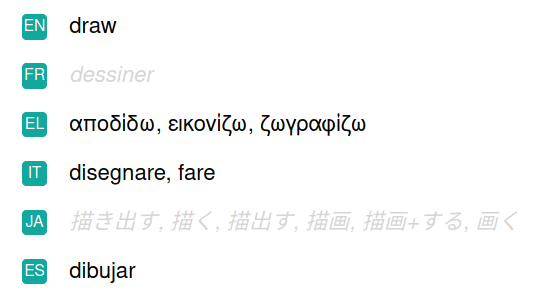
\includegraphics[width=1\linewidth]{./img/fare_synset1.png}
			\caption{Gloss: Drawing an artifact}
			\label{fig:sub1}
		\end{subfigure}%
		\begin{subfigure}{.5\textwidth}
			\centering
			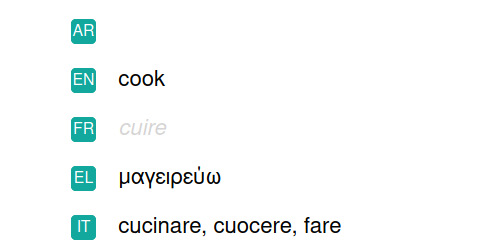
\includegraphics[width=1\linewidth]{./img/fare_synset2.png}
			\caption{Gloss: Transform and make suitable for consumption by heating}
			\label{fig:sub2}
		\end{subfigure}
		\caption{Due Babel-synset in cui compare il lemma "fare". In ogni synset, BabelNet fornisce l'elenco di sinonimi nelle varie lingue ed una definizione (Gloss) del significato sotteso}
		\label{fig:test}
	\end{figure}

Per evitare di dover svolgere Word Sense Disambiguation e quindi di dover analizzare il contesto in cui la parola occorre, sono state fatte le seguenti ipotesi semplificative:
\begin{itemize}
	\item I termini polisemici i cui lemmi appartengono ad $I$ assumono un significato definito a priori e non dipendente dal contesto 
	\item La \textbf{traduzione} dei lemmi è una relazione funzionale ed ovunque definita $R$  tra gli elementi di $I$ ed i lemmi della lingua inglese appartenenti all'insieme denotato con $E$. Ovvero vale la seguente condizione:
	\begin{align*}
		\forall x \in I \quad  \exists! y \in E \quad t.c. \; (x,y) \in R 
	\end{align*}
\end{itemize}
In questo modo per la traduzione possiamo ricorrere ad un dizionario isomorfo italiano-inglese, implementabile in Java con un HashMap.
	\lstinputlisting[label={dizionario},style = javacode, caption ={Dizionario isomorfo IT->EN}]{java/Dizionario}  
Nel Transfer lessicale, visitiamo ciascun nodo dell'albero tramite ricerca in ampiezza, ed estraiamo il lemma della parola associata al nodo. \\
In generale, viene tradotto direttamente l'intero lemma utilizzando il dizionario sopra definito.
Tuttavia, nel caso in cui la parola fosse una preposizione, anziché tradurre direttamente l'intero lemma, traduciamo i morfemi con l'uso del suddetto dizionario e poniamo uno spazio tra i morfemi tradotti per generare il risultato.
Ad esempio, data la preposizione "della", individuiamo i morfemi "del-la" derivanti dall'analisi morfologica. Traduciamo quindi i singoli morfermi (del->of, la->the) in modo da ottenere la traduzione "of the". \\
Il risultato della traduzione viene salvato in un attributo del nodo corrente visitato.
\subsection{Transfer sintattico}
\label{sec:transfer_sintattico}
Il processo di generazione, che rappresenta la fase finale della nostra pipeline di elaborazione (Fig. \ref{Vauquois_triangle}), è affidato alla libreria Java SimpleNLG \cite{simpleNLG}, un \textbf{realizzatore linguistico} che utilizzando regole grammaticali dell'inglese (morfologiche e sintattiche) converte la rappresentazione astratta della frase (\textbf{sentence plan ibrido}) data in input in testo effettivo. \\

Pertanto, nel nostro caso il ruolo del Transfer Sintattico è quello di fungere da ponte tra l'albero a dipendenze finora discusso ed il sentence plan ibrido richiesto in input da SimpleNLG.
\begin{figure}[ht]
	\centering 
	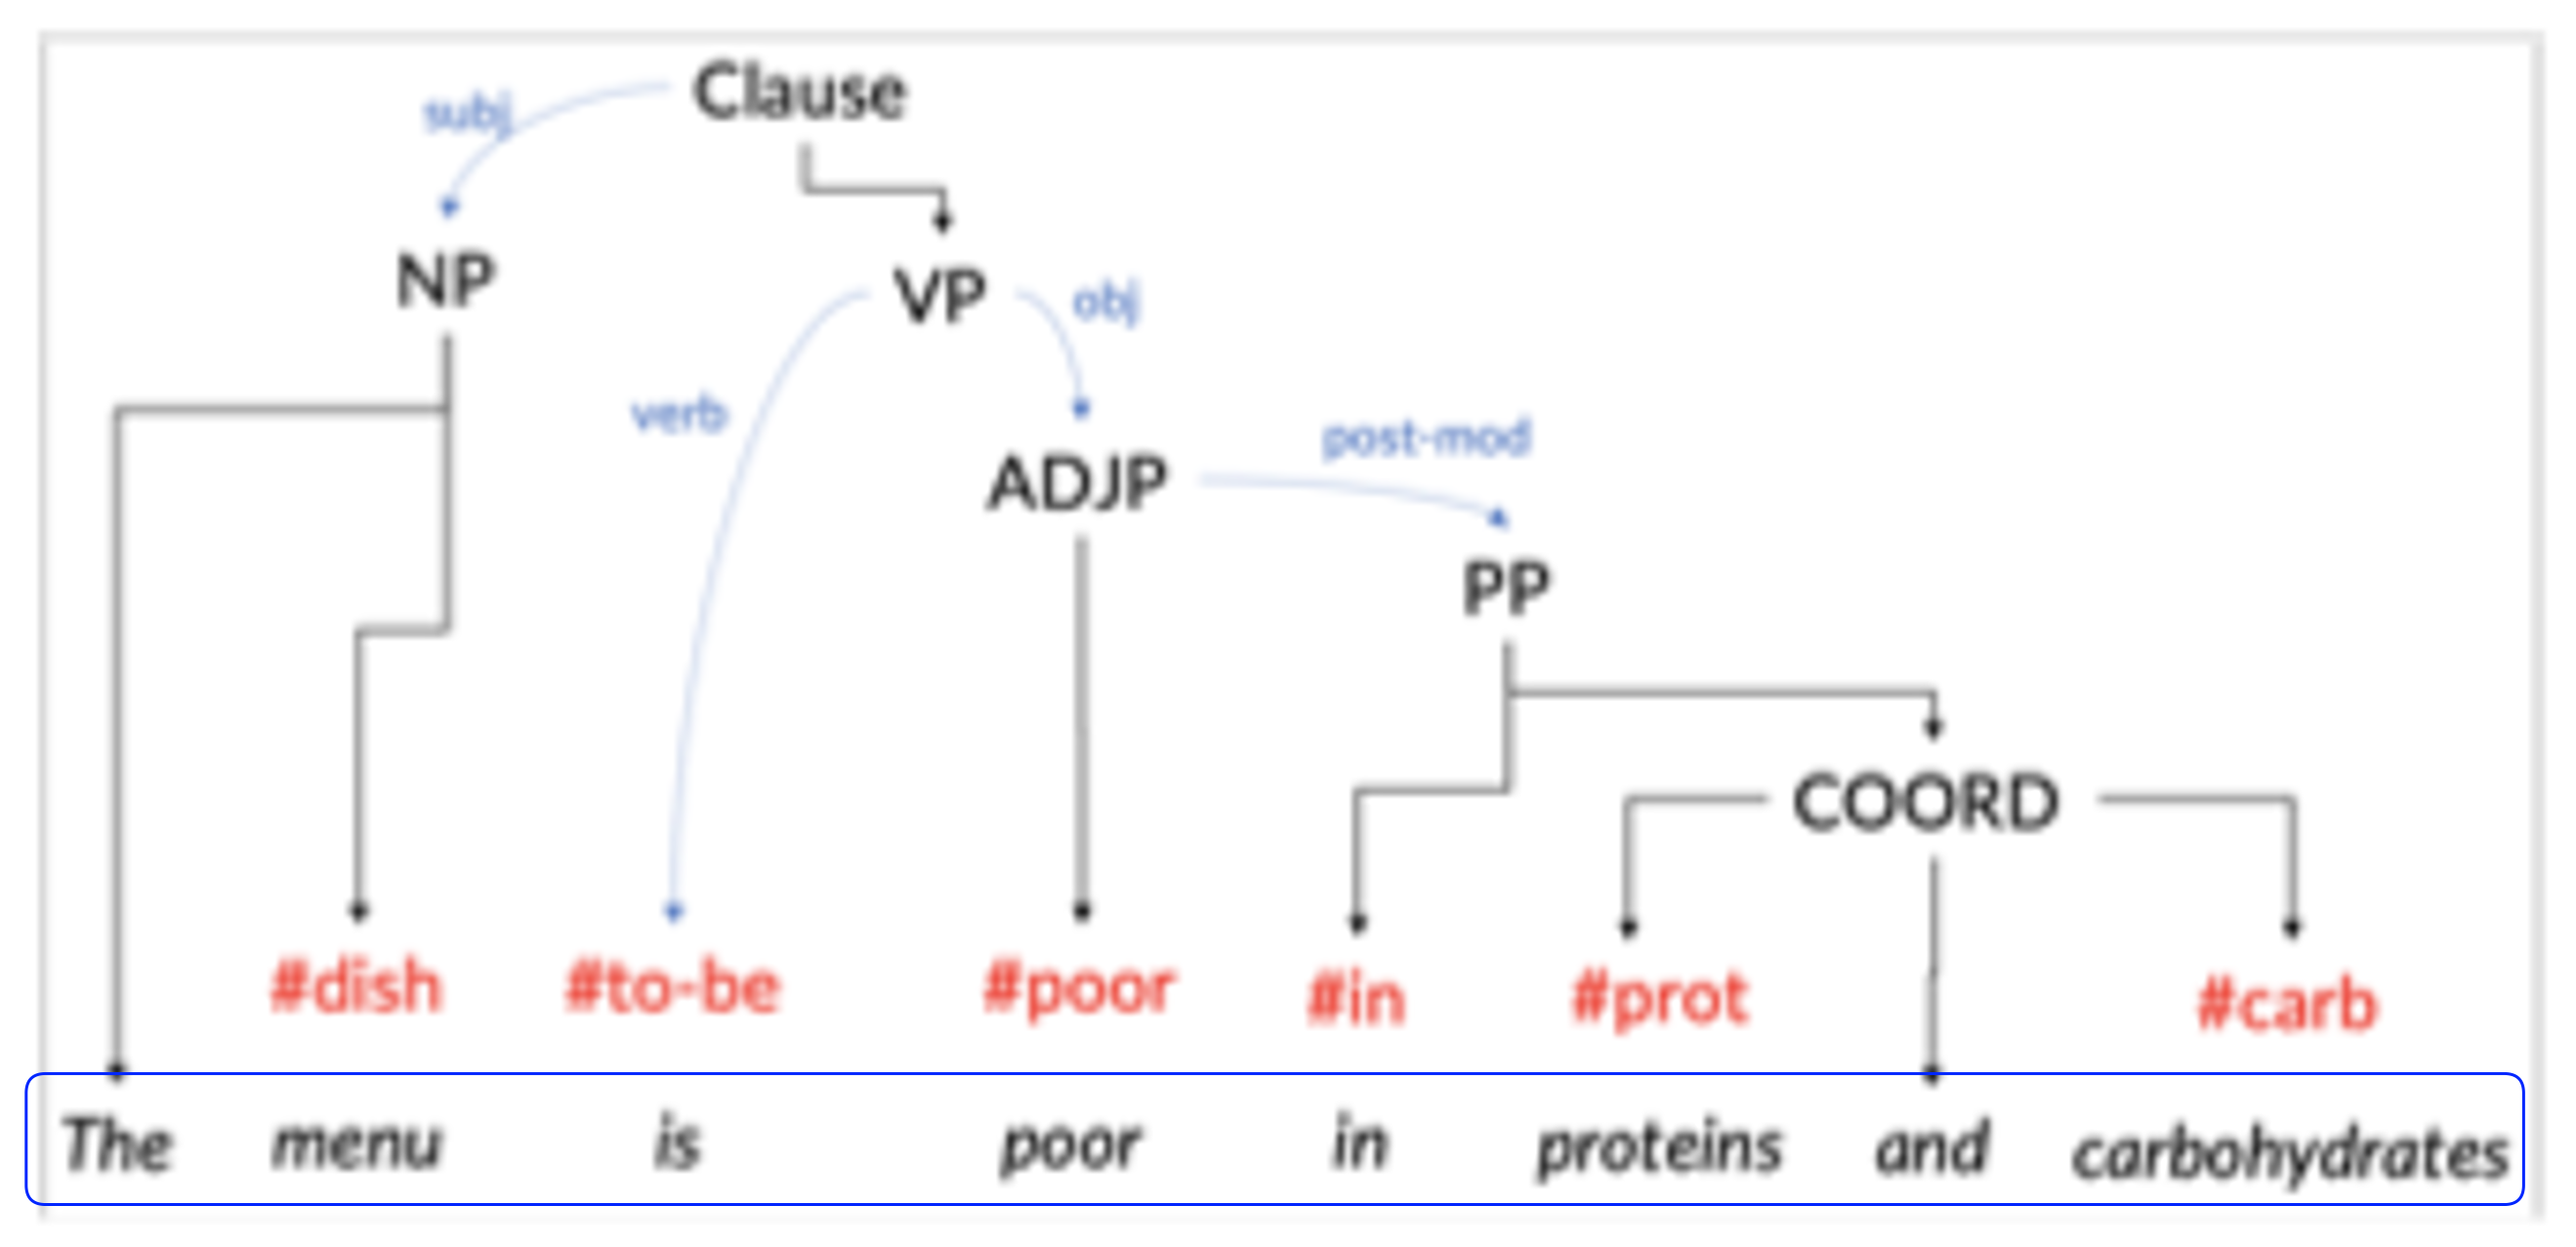
\includegraphics[width=1\linewidth]{./img/sentence_plan}
	\caption{Nella parte alta viene raffigurato un sentence plan ibrido, nell'ultimo livello viene presentato il risultato della realizzazione linguistica (testo)}
	\label{sentence_plan}
\end{figure} \\
Ci limitiamo a fare alcune considerazioni sulle peculiarità di quest'ultima struttura dati citata, considerando l'esempio in Figura 5:
\begin{itemize}
	\item Vi sono relazioni binarie asimmetriche grammaticali tra la frase ed i costituenti. \\Nell'esempio la relazione \textit{subj} lega la frase ad un NP (sintagma nominale)
	\item Si può specificare relazioni binarie asimmetriche grammaticali anche tra i costituenti. \\Nell'esempio la relazione \textit{post-mod} lega il sintagma aggettivale (dominante) ad un PP (modificatore ).	
	\item Le foglie dell'albero ospitano i lemmi in lingua inglese. Sarà compito di SimpleNLG effettuare la generazione morfologica sulla base delle informazioni linguistiche fornite (ad esempio, se il soggetto è in terza persona singolare ed il tempo verbale è al presente, verrà aggiunto il suffisso "-s" al verbo)
	\item In questa rappresentazione astratta della frase, l'ordine delle parole non c'è in quanto sarà stabilito da SimpleNLG al momento della generazione, in maniera conforme alle regole morfo-sintattiche dell'inglese
\end{itemize}
		\begin{figure}[ht]
		\centering
		\begin{subfigure}{.4\textwidth}
			\centering
			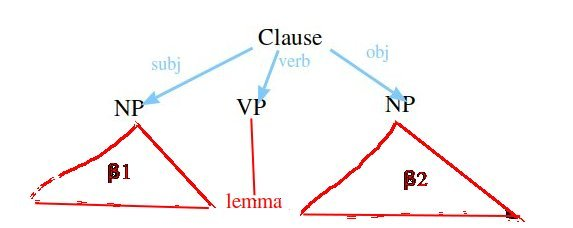
\includegraphics[width=1\linewidth]{./img/fase2_transfer}
			\caption{Sentence plan ibrido}
			\label{fig:tree_transfer}
		\end{subfigure}%
		\begin{subfigure}{.6\textwidth}
			\centering
			\lstinputlisting[label={transfer},style = javacode, caption ={}]{java/Fase2Transfer.java}  
			\caption{Snippet di codice costruzione sentence-plan ibrido a partire dall'albero a dipendenze}
			\label{fig:code_transfer}
		\end{subfigure}
		\caption{Da una parte porzione del codice utilizzato per trasformare l'albero a dipendenze in un sentence plan. Dall'altra rappresentazione grafica della struttura dati generata. }
		\label{fig:transfer}
	\end{figure}
Descriviamo ora il processo di trasformazione dell'albero a dipendenze in sentence plan ibrido,
supponendo che la frase in ingresso sia in forma attiva e che il verbo sia transitivo\footnote{NOTA BENE: per rendere l'esposizione più chiara, la descrizione si è focalizzata al caso in cui la frase fosse attiva ed il verbo transitivo. Tuttavia, il programma dispone di opportune regole per gestire casi relativi a frasi in forma passiva, predicati nominali, ... etc.}.. \\

In primo luogo, si esaminano i nodi dell'albero a dipendenze posti ad una profondità massima di 1 per determinare le relazioni grammaticali della frase (\textit{subj}, \textit{verb}, \textit{obj}) che sono di interesse per il sentence plan ibrido (Figura \ref{fig:transfer} (a)).
Ognuna di queste relazioni coinvolge un opportuno costituente: si costruisce il sotto-albero sotteso (nell'esempio $\beta_1$ per il soggetto, $\beta_2$ per il complemento oggetto) richiamando la funzione  \textit{generatePhrase} (Listing \ref{fig:transfer} (b)) passandogli il nodo dell'albero a dipendenze appena visitato. La funzione tratta tale nodo come una radice di un sotto-albero, che verrà visitato nell'ottica di ottenere le informazioni utili per generare il sotto-albero del sentence plan ibrido.
\\Inoltra, una peculiarità della funzione \textit{generatePhrase} è quella di riuscire a gestire la seguente ricorsione:
			\[ NP \longrightarrow Det \; Noun \;PP \; | \; Det \; Noun \]
			\[ PP \longrightarrow Prep \; NP  \]	
\begin{figure}[ht]
	\centering 
	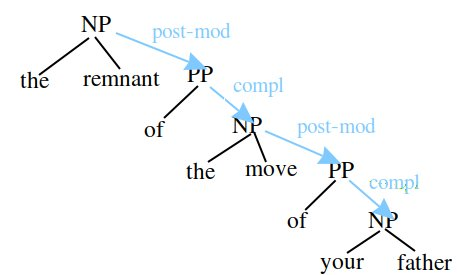
\includegraphics[scale=0.5]{./img/ricorsione}
	\caption{Struttura ricorsiva nel sentence plan ibrido}
	\label{sentence_plan}
\end{figure}
Una volta costruito il sentence plan, SimpleNLG si occuperà di generare la frase per l'inglese, come già discusso all'inizio di questa sezione.

		
							







%	\section{Generazione}
	\section{Conclusioni}
Sono stati svolti gli esperimenti di traduzione su quattro frasi, come mostrato in Figura \ref{console}.
\begin{figure}[ht]
	\centering 
	\lstinputlisting[label={console},style = javacode, caption ={}]{java/console}  
	\caption{Console Java durante esecuzione del programma}
	\label{console}
\end{figure}
\\ Possiamo quindi concludere dicendo che l'approccio simbolico basato su TransferSintattico ha generato buoni risultati. \\
La Neural Machine Translation oggigiorno è il modello attualmente più in voga date le sue performances, tuttavia necessita di molti dati a disposizione, sotto forma ad esempio di pagine multi-lingua da cui poter apprendere. Gli approcci simbolici hanno il vantaggio di basarsi esclusivamente su regole, quindi si può sulla carta tradurre anche lingue poco diffuse sul Web. Inoltre, nelle reti neurali
le decisioni prese della macchina non sono trasparenti e spesso incomprensibili anche agli occhi degli esperti, mentre negli approcci simbolici i processi di che hanno portato ad un determinato output sono interpretabili e direttamente correggibili in caso di problemi.

	\newpage
	\bibliographystyle{alpha}
	\bibliography{biblio.bib}

\end{document} % NOTHING AFTER THIS LINE IS PART OF THE DO